\documentclass{article}
\usepackage[utf8]{inputenc}
\usepackage[italian]{babel}
\usepackage{amsmath}
\usepackage{amssymb}
\usepackage{siunitx}
\usepackage{tabularray}
\usepackage{graphicx}
\usepackage{float}
% \usepackage{minted}
\usepackage[bottom]{footmisc}
\usepackage[page]{appendix}
\usepackage[labelformat=simple, justification=centering]{subfig}
\renewcommand{\thesubfigure}{}
\newcommand*{\diam}{\varnothing}
\newcommand*{\best}[1]{{#1}_\text{best}}
\newcommand*{\bestp}[1]{{\left(#1\right)}_\text{best}}
\newcommand*{\pbest}[1]{\left({#1}_\text{best}\right)}
\newcommand*{\pbestp}[1]{\left({\left(#1\right)}_\text{best}\right)}
\newcommand*{\errrel}[1]{\frac{\delta #1}{{#1}_\text{best}}}
\title{
  Laboratorio di Fisica 1\\
  R12: Misura della velocità del suono
}
\author{Gruppo 15: Bergamaschi Riccardo, Graiani Elia, Moglia Simone}
\date{28/05/2024 – 04/06/2024}
\makeindex
\begin{document}

\maketitle

\begin{abstract}
  Il gruppo di lavoro ha misurato la velocità del suono mediante
  lo studio di onde stazionarie in una colonna d'aria.
\end{abstract}

\setcounter{section}{-1}
\section{Materiali e strumenti di misura utilizzati}
\begin{center}
\begin{tblr}{
  width=\textwidth,
  colspec={ X[2,m,j]X[1,m,c]X[1,m,c]X[1,m,c] },
  vlines,
}
  \hline
  \textbf{Strumento di misura} & \textbf{Soglia} & \textbf{Portata} & \textbf{Sensibilità} \\
  \hline
  Metro a nastro & $\qty{0.1}{cm}$ & $\qty{300.0}{cm}$ & $\qty{0.1}{cm}$ \\
  \hline[dashed]
  Calibro ventesimale & $\qty{0.05}{mm}$ & $\qty{150.00}{mm}$ & $\qty{0.05}{mm}$ \\
  \hline[dashed]
  Oscilloscopio\footnotemark[1] & $\qty{2.5}{ms}$ & N./A. & $\qty{2.5}{ms}$ \\
  \hline
\end{tblr}
\footnotetext[1]{
  % TODO
}
\begin{tblr}{
  width=\textwidth,
  colspec={ X[m,j]X[3,m,j] },
  vlines,
}
  \hline
  \textbf{Altro} & \textbf{Descrizione/Note} \\
  \hline
  Tubo in plastica & {
    Nel quale facciamo propagare le onde sonore.
  } \\
  \hline[dashed]
  Oscilloscopio & {
    Permette di visualizzare la forma d'onda emessa e quella
    rilevata dal microfono.
  } \\
  \hline[dashed]
  Generatore di funzioni d'onda & {
    Con cui possiamo regolare frequenza, ampiezza e
    forma d'onda delle onde generate.
  } \\
  \hline[dashed]
  Altoparlante & {
    Utilizzato per emettere le onde sonore.
  } \\
  \hline[dashed]
  Microfono a condensatore & {
    Utilizzato per rilevare le onde di pressione.
  } \\
  \hline[dashed]
  Pistone & {
    Finalizzato alla chiusura di un'estremità del tubo.
  } \\
  \hline
\end{tblr}
\end{center}

\pagebreak
\section{Misurazione indiretta mediante le frequenze di risonanza}

\subsection{Esperienza e procedimento di misura}

\begin{enumerate}
  \item
    Con il metro a nastro misuriamo la lunghezza del tubo $L$,
    mentre con il calibro ventesimale il suo diametro interno
    $\diam=(38.20\pm0.05)\,\unit{mm}$.
  \item
    Accesi l'oscilloscopio e il generatore di forme d'onda,
    regoliamo l'ampiezza in modo da poter percepire un suono.
  \item
    Inseriamo il microfono dentro al tubo in modo che riesca a rilevare le onde
    chiaramente, quindi assicurandoci che, in presenza di onde stazionarie,
    non si trovi in corrispondenza di un nodo.
  \item
    Aumentiamo la frequenza fino a trovare, mediante l'oscilloscopio,
    il primo massimo relativo nell'ampiezza del segnale rilevato dal
    microfono: questa sarà la prima frequenza di risonanza,
    ovvero l'armonica fondamentale.
  \item
    Ripetiamo più volte il passaggio precedente, in modo da ottenere le prime
    armoniche (multiple della fondamentale).
\end{enumerate}
Il gruppo di lavoro ha effettuato nuovamente gli stessi passaggi più volte,
mantenendo l'estremità del tubo opposta all'altoparlante chiusa tramite il pistone.
In questo caso la lunghezza del tubo da considerare è quella tra l'estremità
aperta e il pistone.

\subsection{Analisi dei dati raccolti}
\emph{\textbf{Nota.}
Avendo valutato gli errori sulle grandezze misurate direttamente
come piccoli, casuali e indipendenti, per svolgere ogni calcolo
abbiamo utilizzato la tradizionale propagazione degli errori.
}
\vspace{2mm}

La frequenza emessa è una delle frequenze di risonanza del tubo se e solo se
all'interno di quest'ultimo si forma un'onda stazionaria. In tal caso:
\begin{itemize}
  \item se il tubo è aperto a entrambi gli estremi,
    lì la pressione è costante (quella atmosferica) e si formano due nodi.
    La lunghezza d'onda sarà allora della forma:
    \[ \lambda_n^\text{a} = \frac{2L}{n},\quad n\in\mathbb{N} \]
  \item se invece il tubo è chiuso ad un estremo,
    lì si forma un ventre, mentre all'altro estremo (dove la pressione è
    quella atmosferica, costante) si forma un nodo:
    \[ \lambda_n^\text{c} = \frac{4L}{n},\quad n\in\mathbb{N}\;\text{dispari} \]
\end{itemize}

Tuttavia, non trattandosi di nodi e ventri ideali, è necessario effettuare
una correzione empirica:

\begin{center}\begin{tblr}{
  colspec={ X[m,c,$$]X[m,c,$$] },
  width=\textwidth,
  hspan=even,
}
  \lambda_n^\text{a} = \frac{2L + 1.6 \diam}{n},\quad n\in\mathbb{N};
  &
  \lambda_n^\text{c} = \frac{4L + 1.6 \diam}{n},\quad n\in\mathbb{N}\;\text{dispari}
\end{tblr}\end{center}
Moltiplicando ambo i membri per la rispettiva frequenza di risonanza
($\nu_n^\text{a}$ o $\nu_n^\text{c}$)
e ricordando che $\lambda_n^\text{a}\,\nu_n^\text{a} =
\lambda_n^\text{c}\,\nu_n^\text{c} = v$, la velocità del suono:

\begin{center}\begin{tblr}{
  colspec={ X[m,c,$$]X[m,c,$$] },
  width=\textwidth,
  hspan=even,
}
  v = \frac{\nu_n^\text{a}}{n}(2L + 1.6 \diam),\quad n\in\mathbb{N};
  &
  v = \frac{\nu_n^\text{c}}{n}(4L + 1.6 \diam),\quad n\in\mathbb{N}\;\text{dispari}
\end{tblr}\end{center}

Riarrangiando i termini, si ottiene:

\begin{center}\begin{tblr}{
  colspec={ X[m,c,$$]X[m,c,$$] },
  width=\textwidth,
  hspan=even,
}
  \nu_n^\text{a} = \xi^\text{a} n,\quad n\in\mathbb{N};
  &
  \nu_n^\text{c} = \xi^\text{c} n,\quad n\in\mathbb{N}\;\text{dispari}
\end{tblr}\end{center}
avendo posto, rispettivamente:

\begin{center}\begin{tblr}{
  colspec={ X[m,c,$$]X[m,c,$$] },
  width=\textwidth,
  hspan=even,
}
  \xi^\text{a} = \frac{v}{2L + 1.6 \diam};
  &
  \xi^\text{c} = \frac{v}{4L + 1.6 \diam}
\end{tblr}\end{center}

Poiché la dipendenza di $\nu_n$ da $n$ è, in entrambi i casi,
di proporzionalità diretta, per determinare $\xi^\text{a}$
e $\xi^\text{c}$ il gruppo di lavoro ha effettuato, per ogni
valore di $L$, una regressione lineare.

Di seguito riportiamo, in grafico, i dati raccolti, accompagnati
dalle rispettive rette di regressione e dai valori di $L$,
$\xi$ e $v$ ottenuti.

\begin{figure}[H]
  \centering
  \subfloat[][
    $L=(90.0\pm0.1)\;\unit{cm}$ \\
    $\xi^\text{a}=(187.004\pm0.008)\unit{Hz}$ \\
    $v=(348.0\pm0.5)\,\unit{m \per s}$
  ]{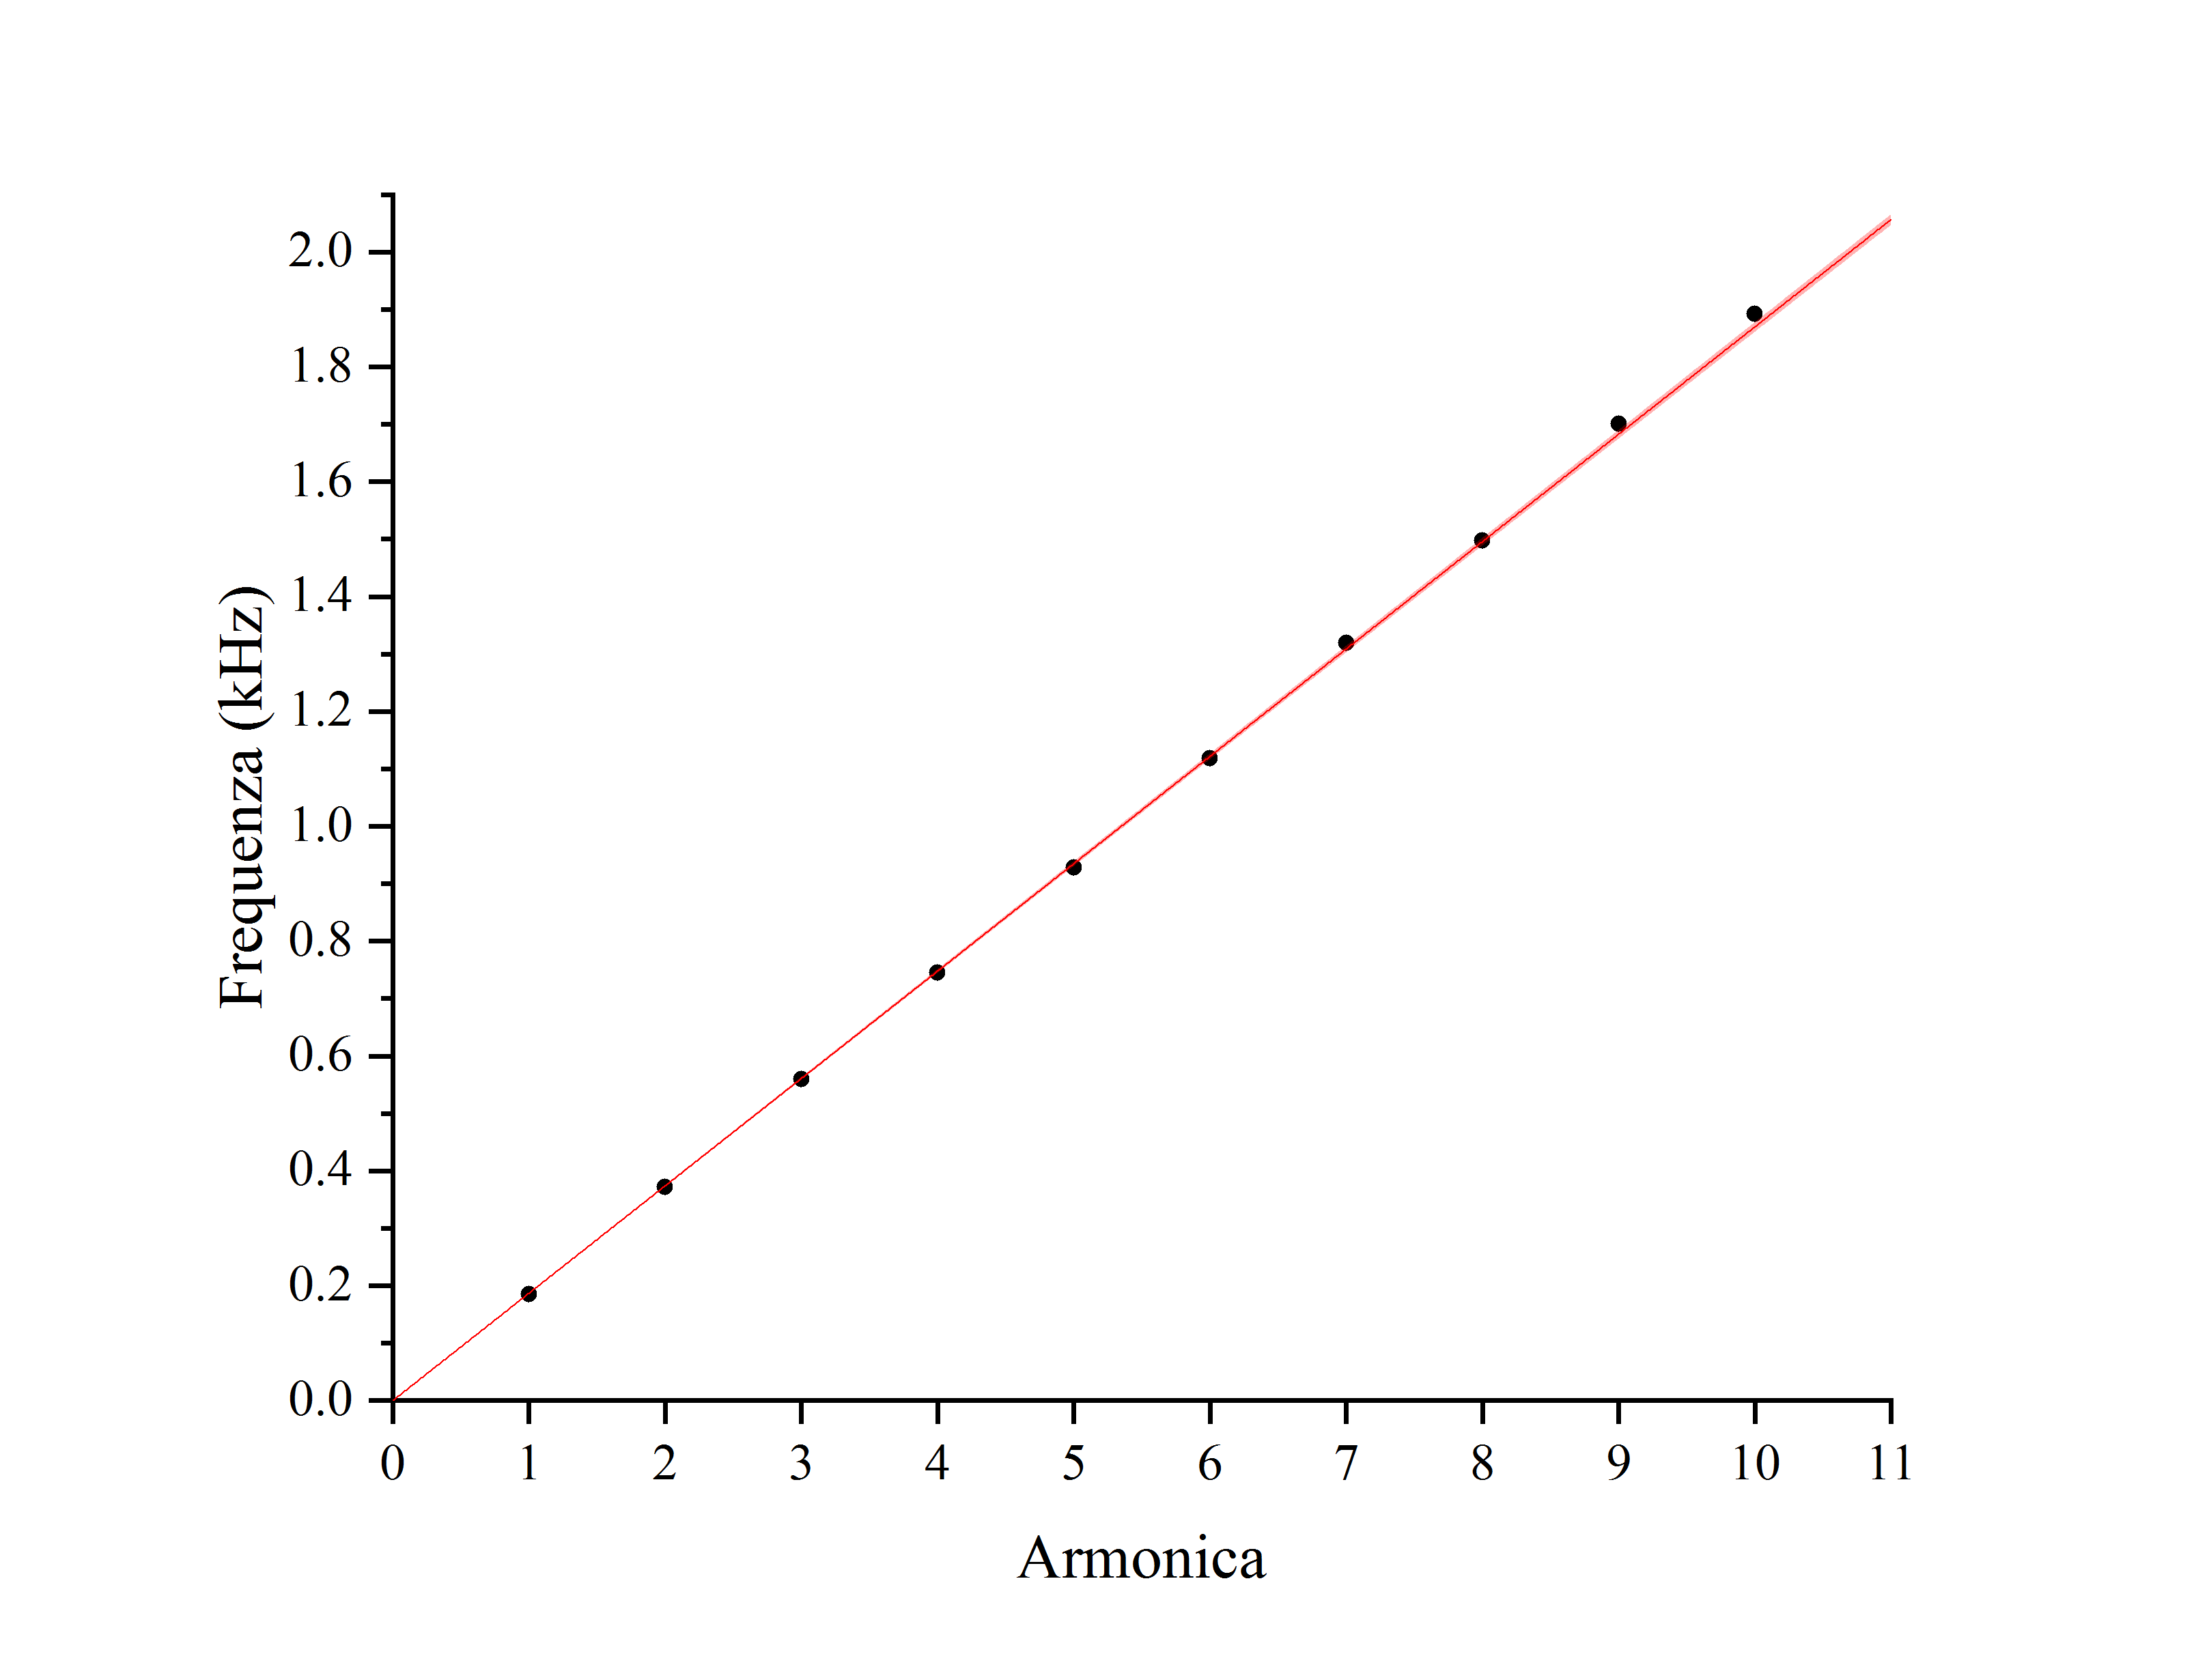
\includegraphics[trim={2.1cm 0.7cm 2.1cm 2cm},clip,width=0.47\textwidth]{img/l0r4.png}}\hfil
\end{figure}\begin{figure}[H]
  \centering
  \subfloat[][
    $L=(71.3\pm0.1)\;\unit{cm}$ \\
    $\xi^\text{c}=(118.64\pm0.06)\unit{Hz}$ \\
    $v=(345.6\pm0.6)\,\unit{m \per s}$
  ]{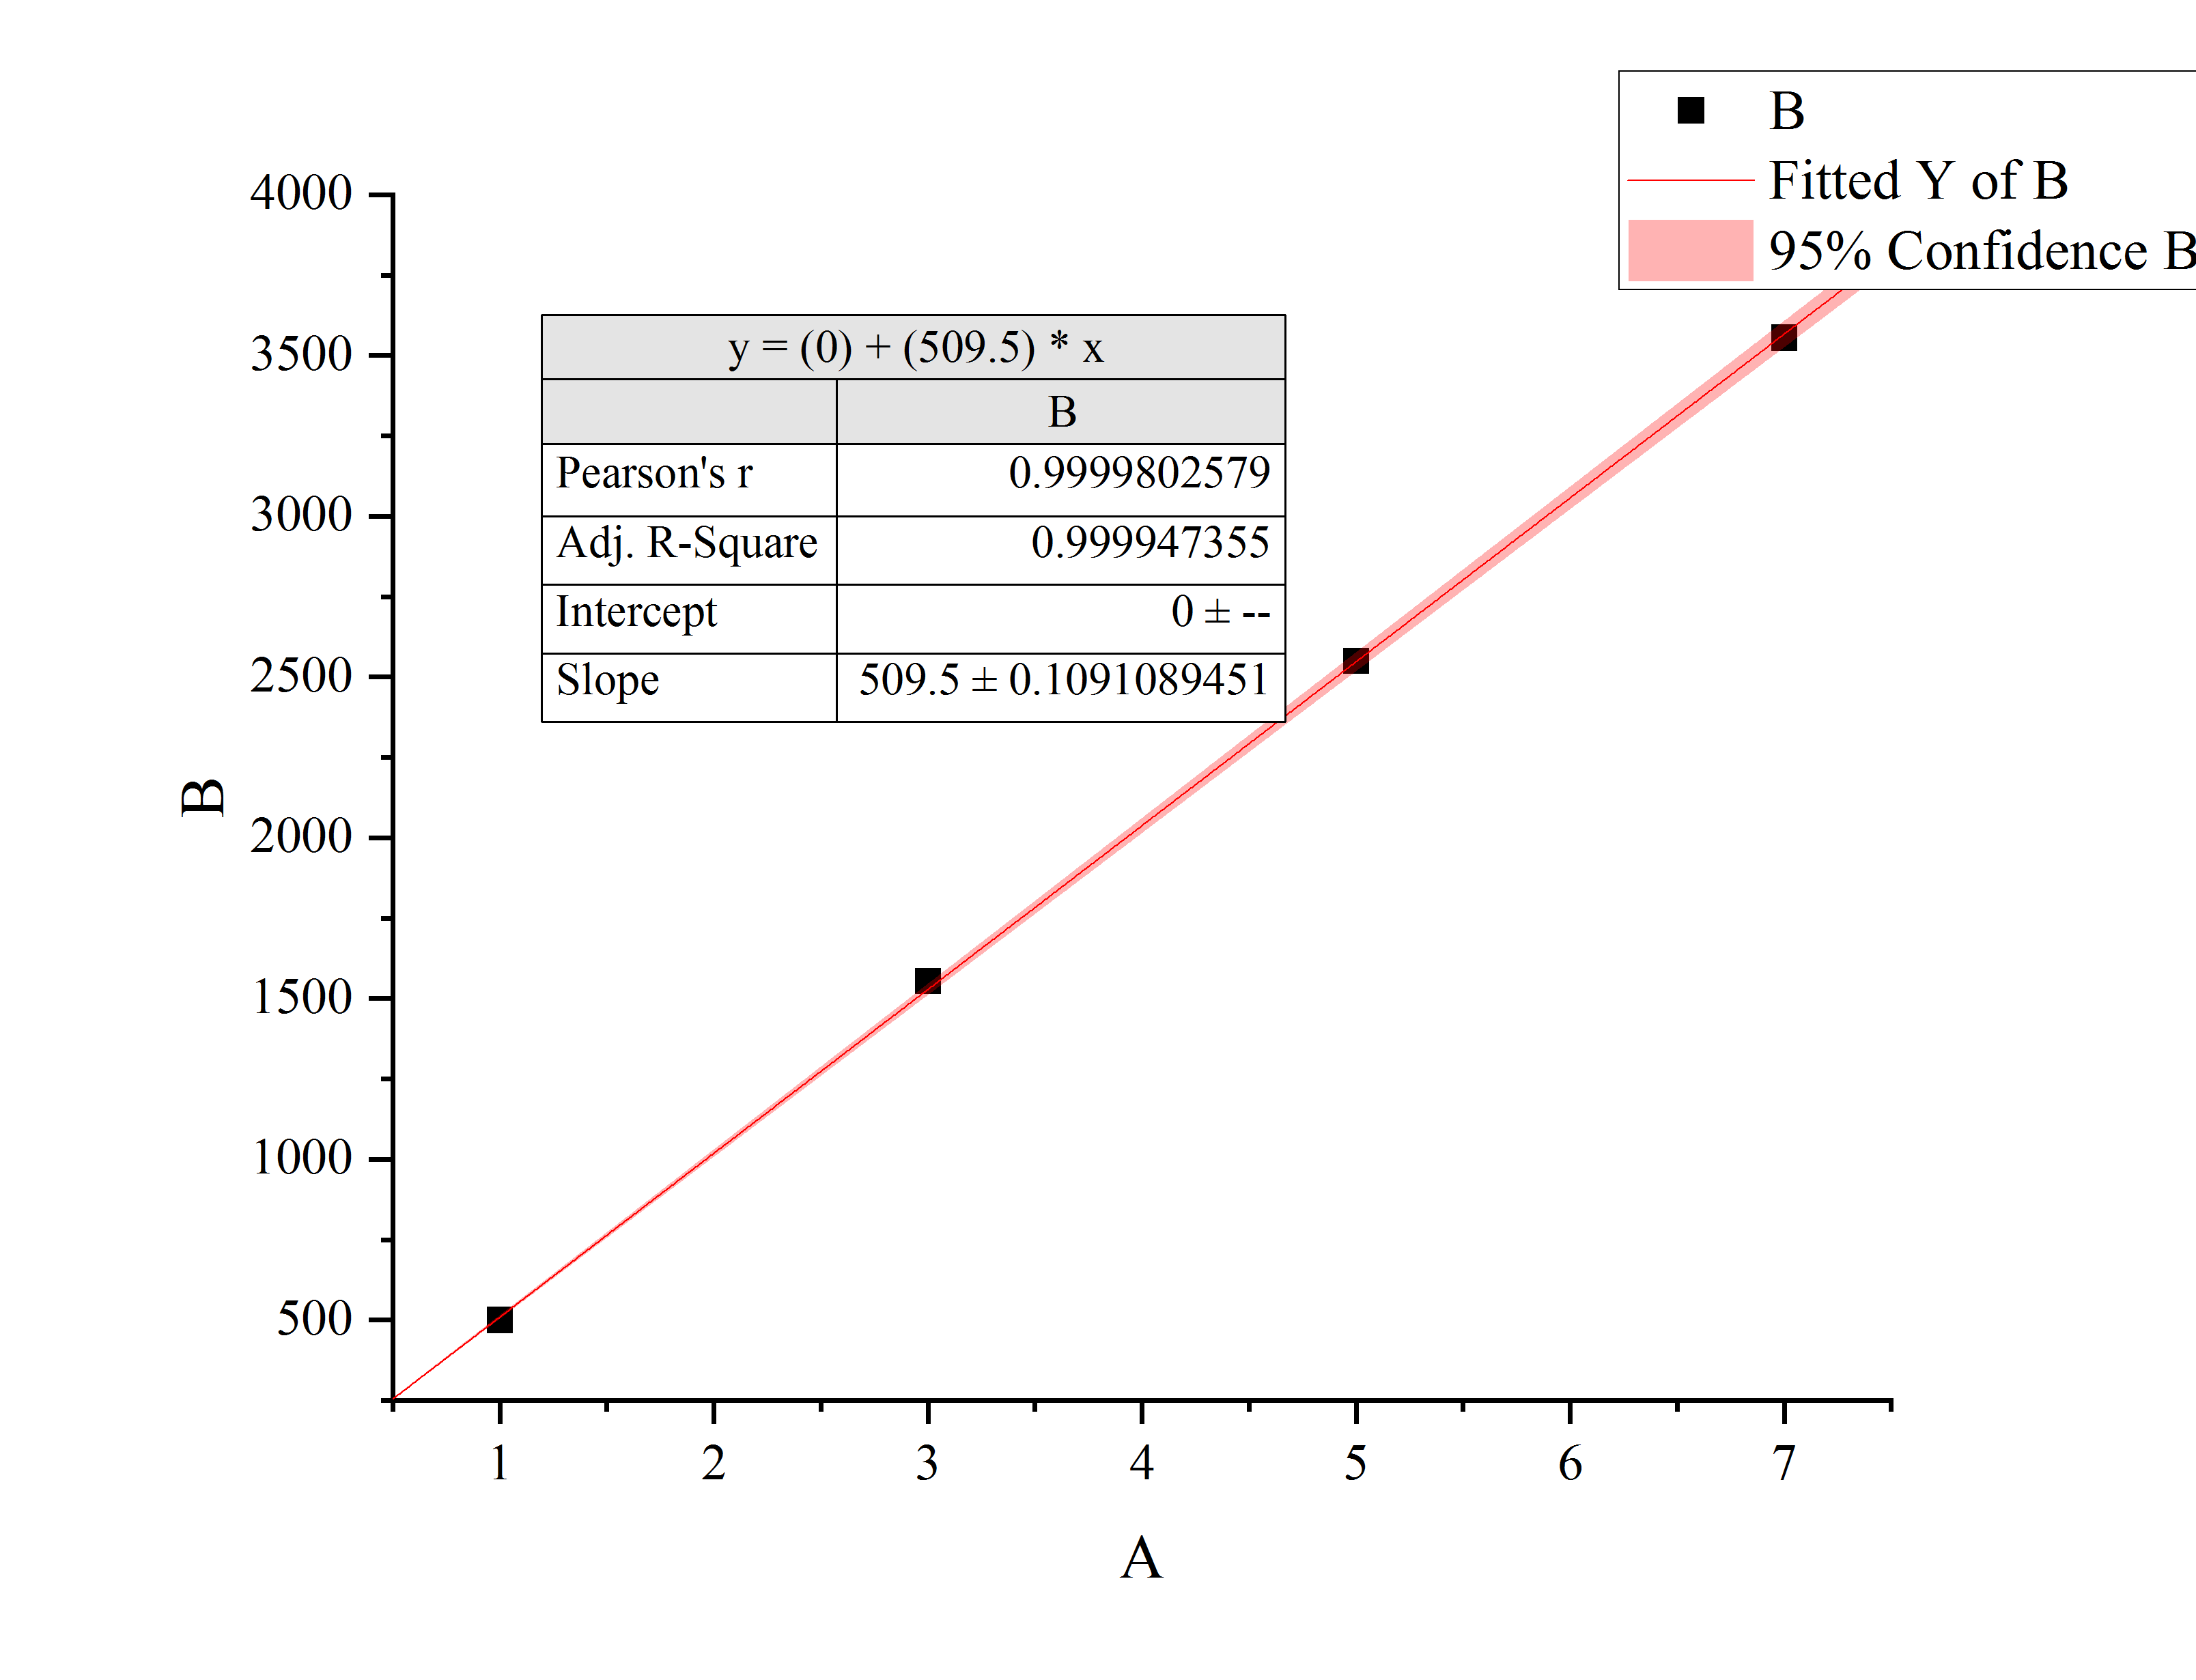
\includegraphics[trim={2.1cm 0.7cm 2.1cm 2cm},clip,width=0.47\textwidth]{img/l1.png}}\hfil
  \subfloat[][
    $L=(55.4\pm0.1)\;\unit{cm}$ \\
    $\xi^\text{c}=(152.12\pm0.06)\unit{Hz}$ \\
    $v=(346.4\pm0.7)\,\unit{m \per s}$
  ]{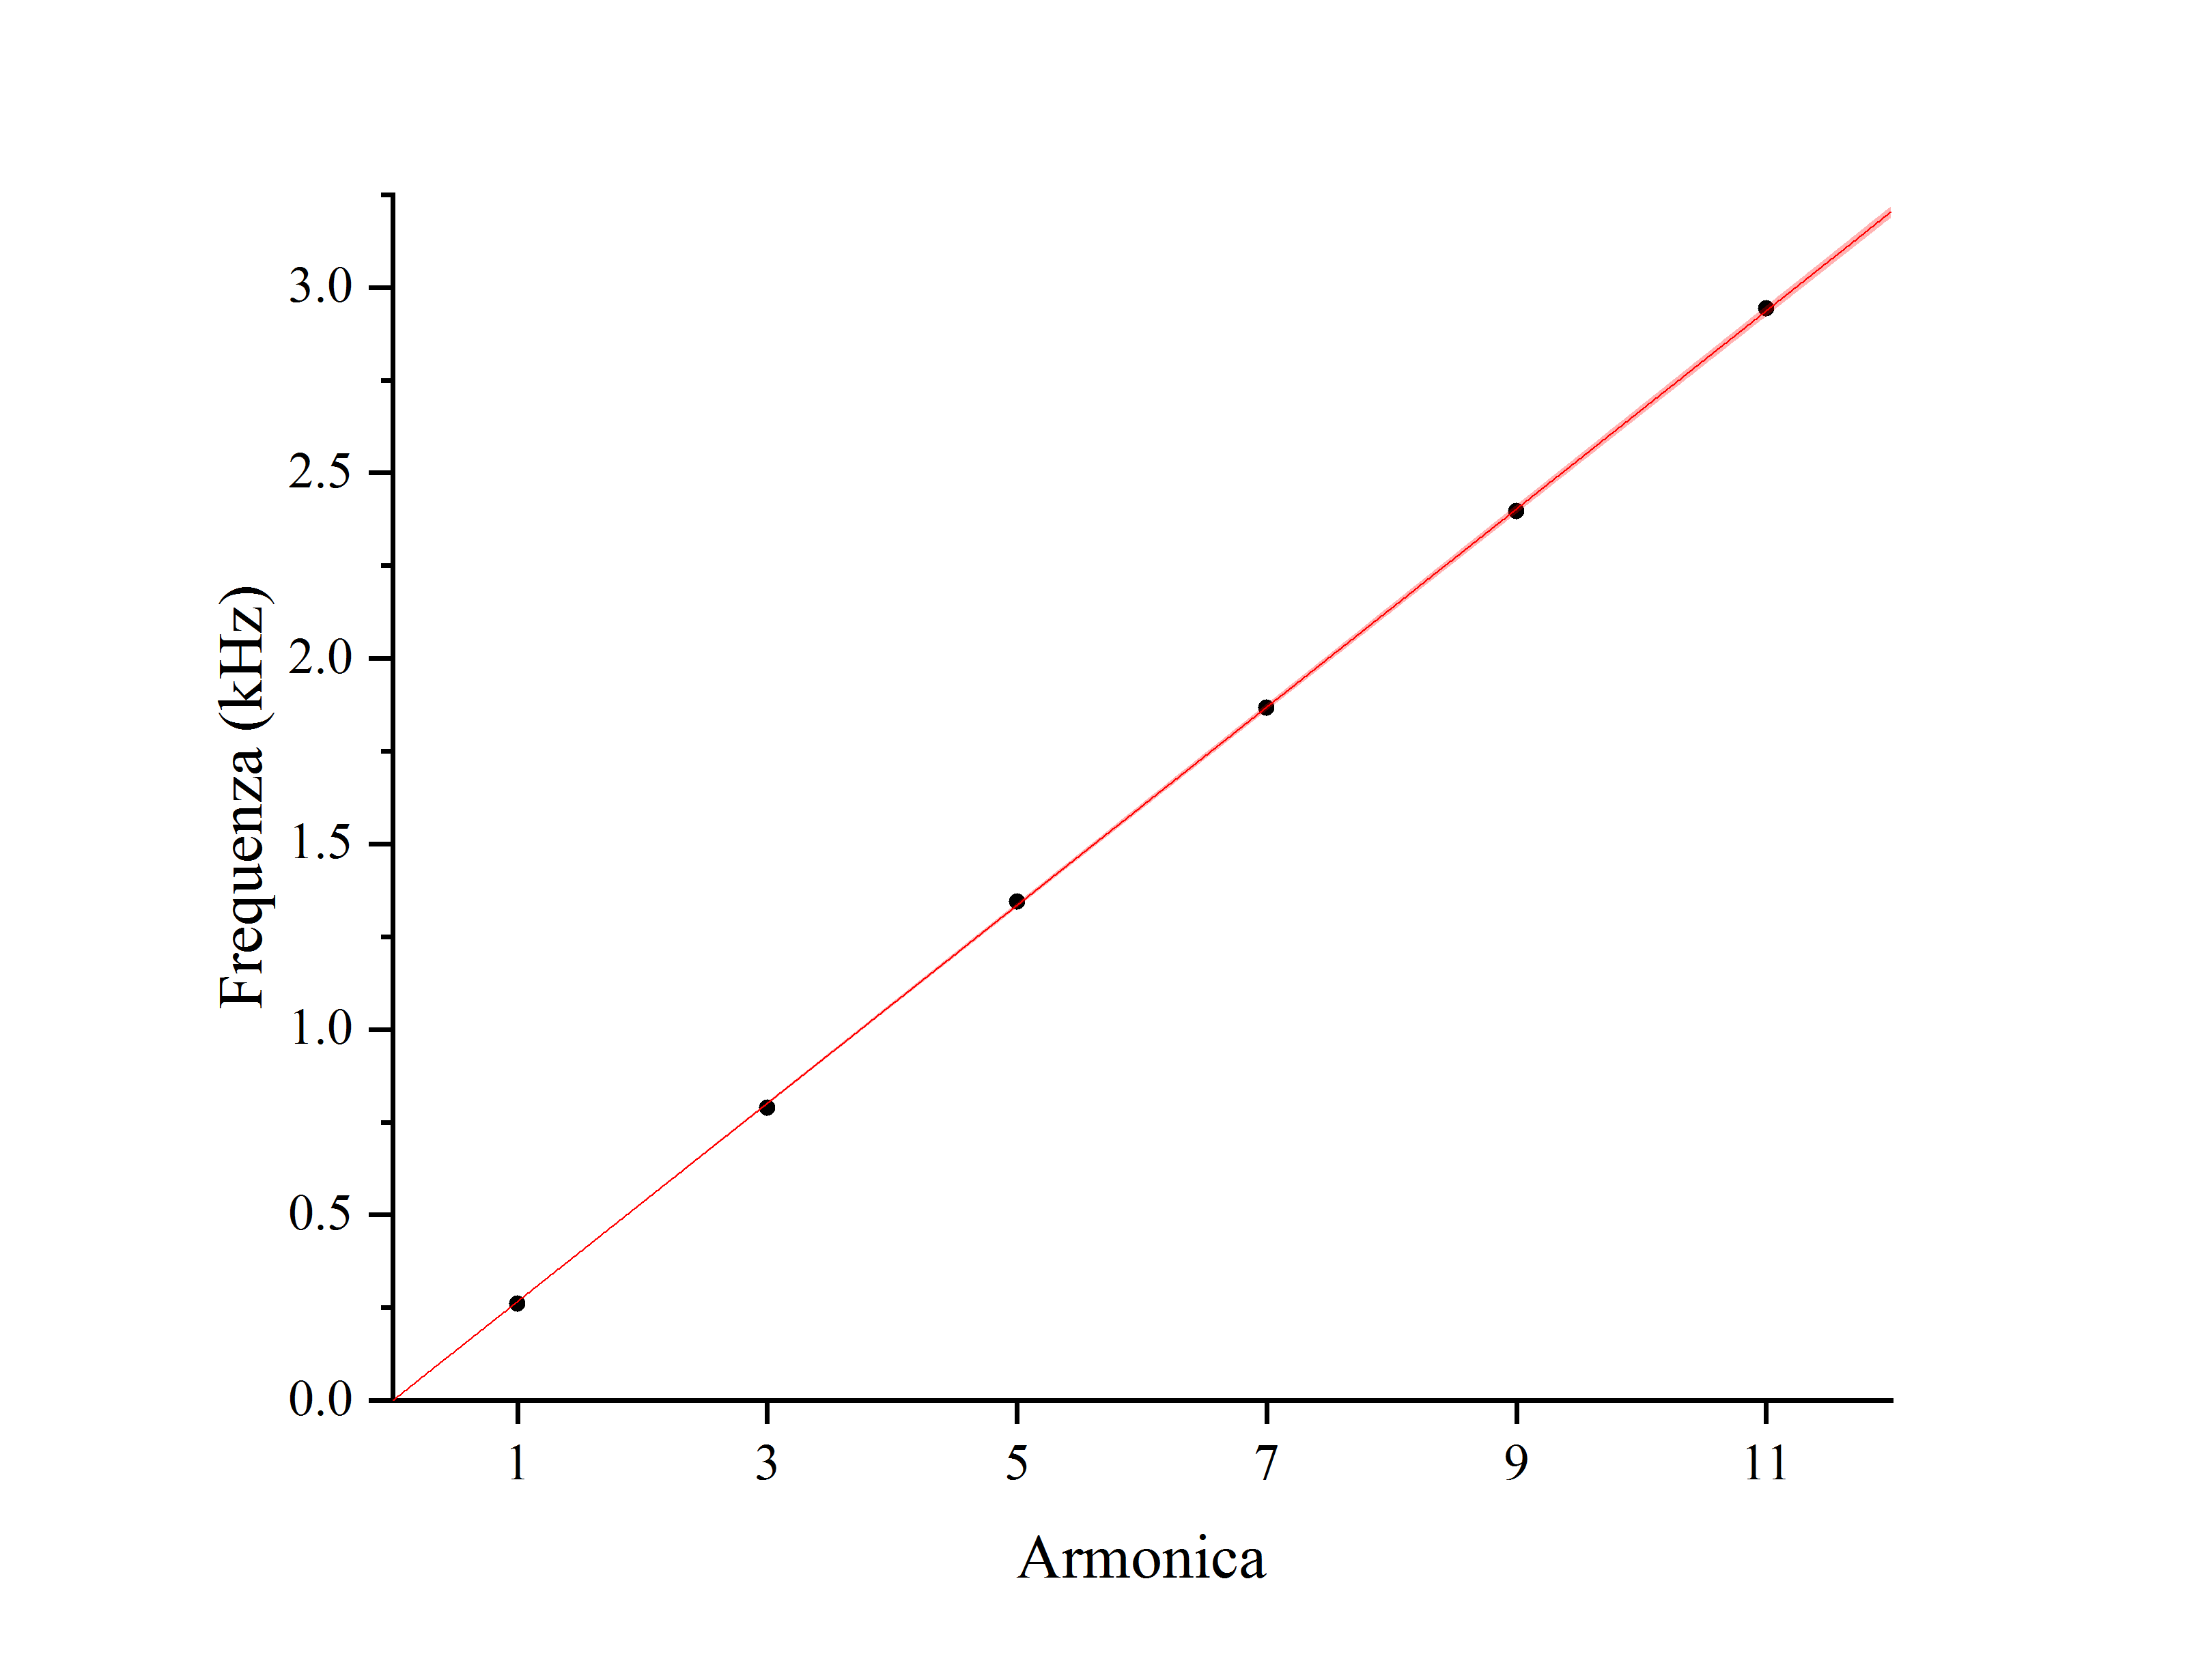
\includegraphics[trim={2.1cm 0.7cm 2.1cm 2cm},clip,width=0.47\textwidth]{img/l2.png}}\hfil
  \subfloat[][
    $L=(30.8\pm0.1)\;\unit{cm}$ \\
    $\xi^\text{c}=(267.00\pm0.06)\unit{Hz}$ \\
    $v=(345.3\pm1.1)\,\unit{m \per s}$
  ]{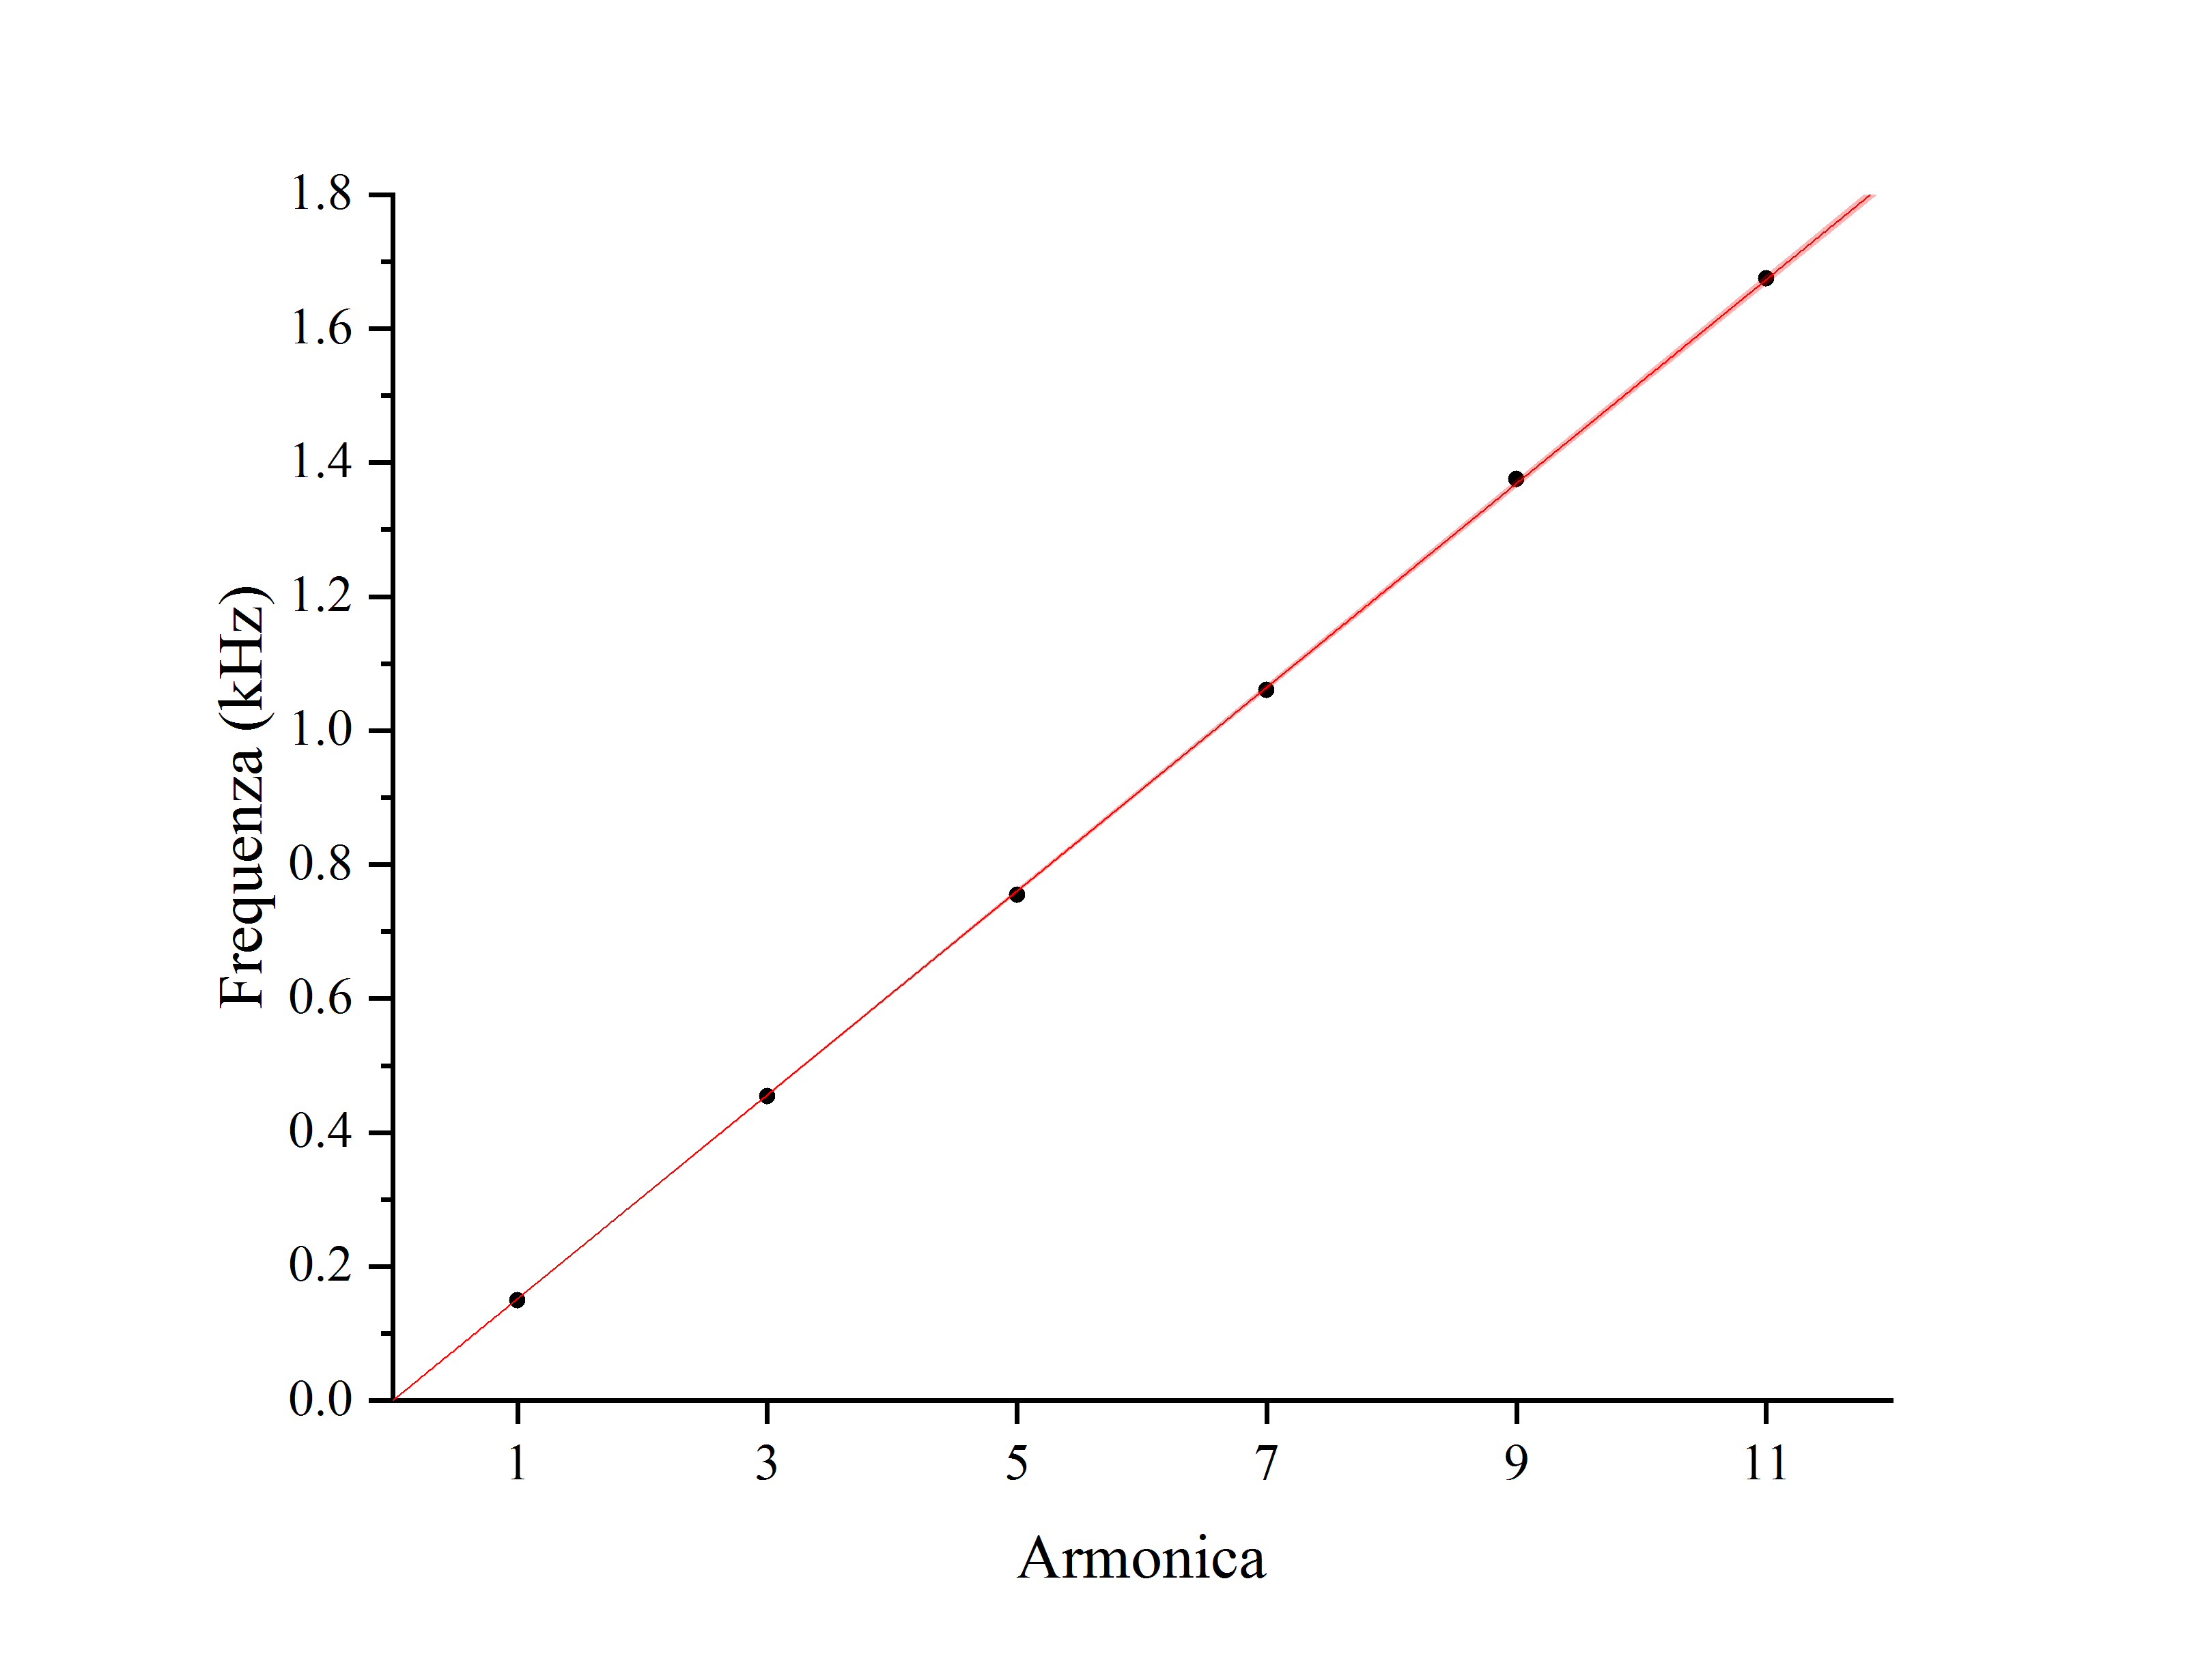
\includegraphics[trim={2.1cm 0.7cm 2.1cm 2cm},clip,width=0.47\textwidth]{img/l3.png}}\hfil
  \subfloat[][
    $L=(15.4\pm0.1)\;\unit{cm}$ \\
    $\xi^\text{c}=(509.5\pm0.1)\unit{Hz}$ \\
    $v=(345\pm2)\,\unit{m \per s}$
  ]{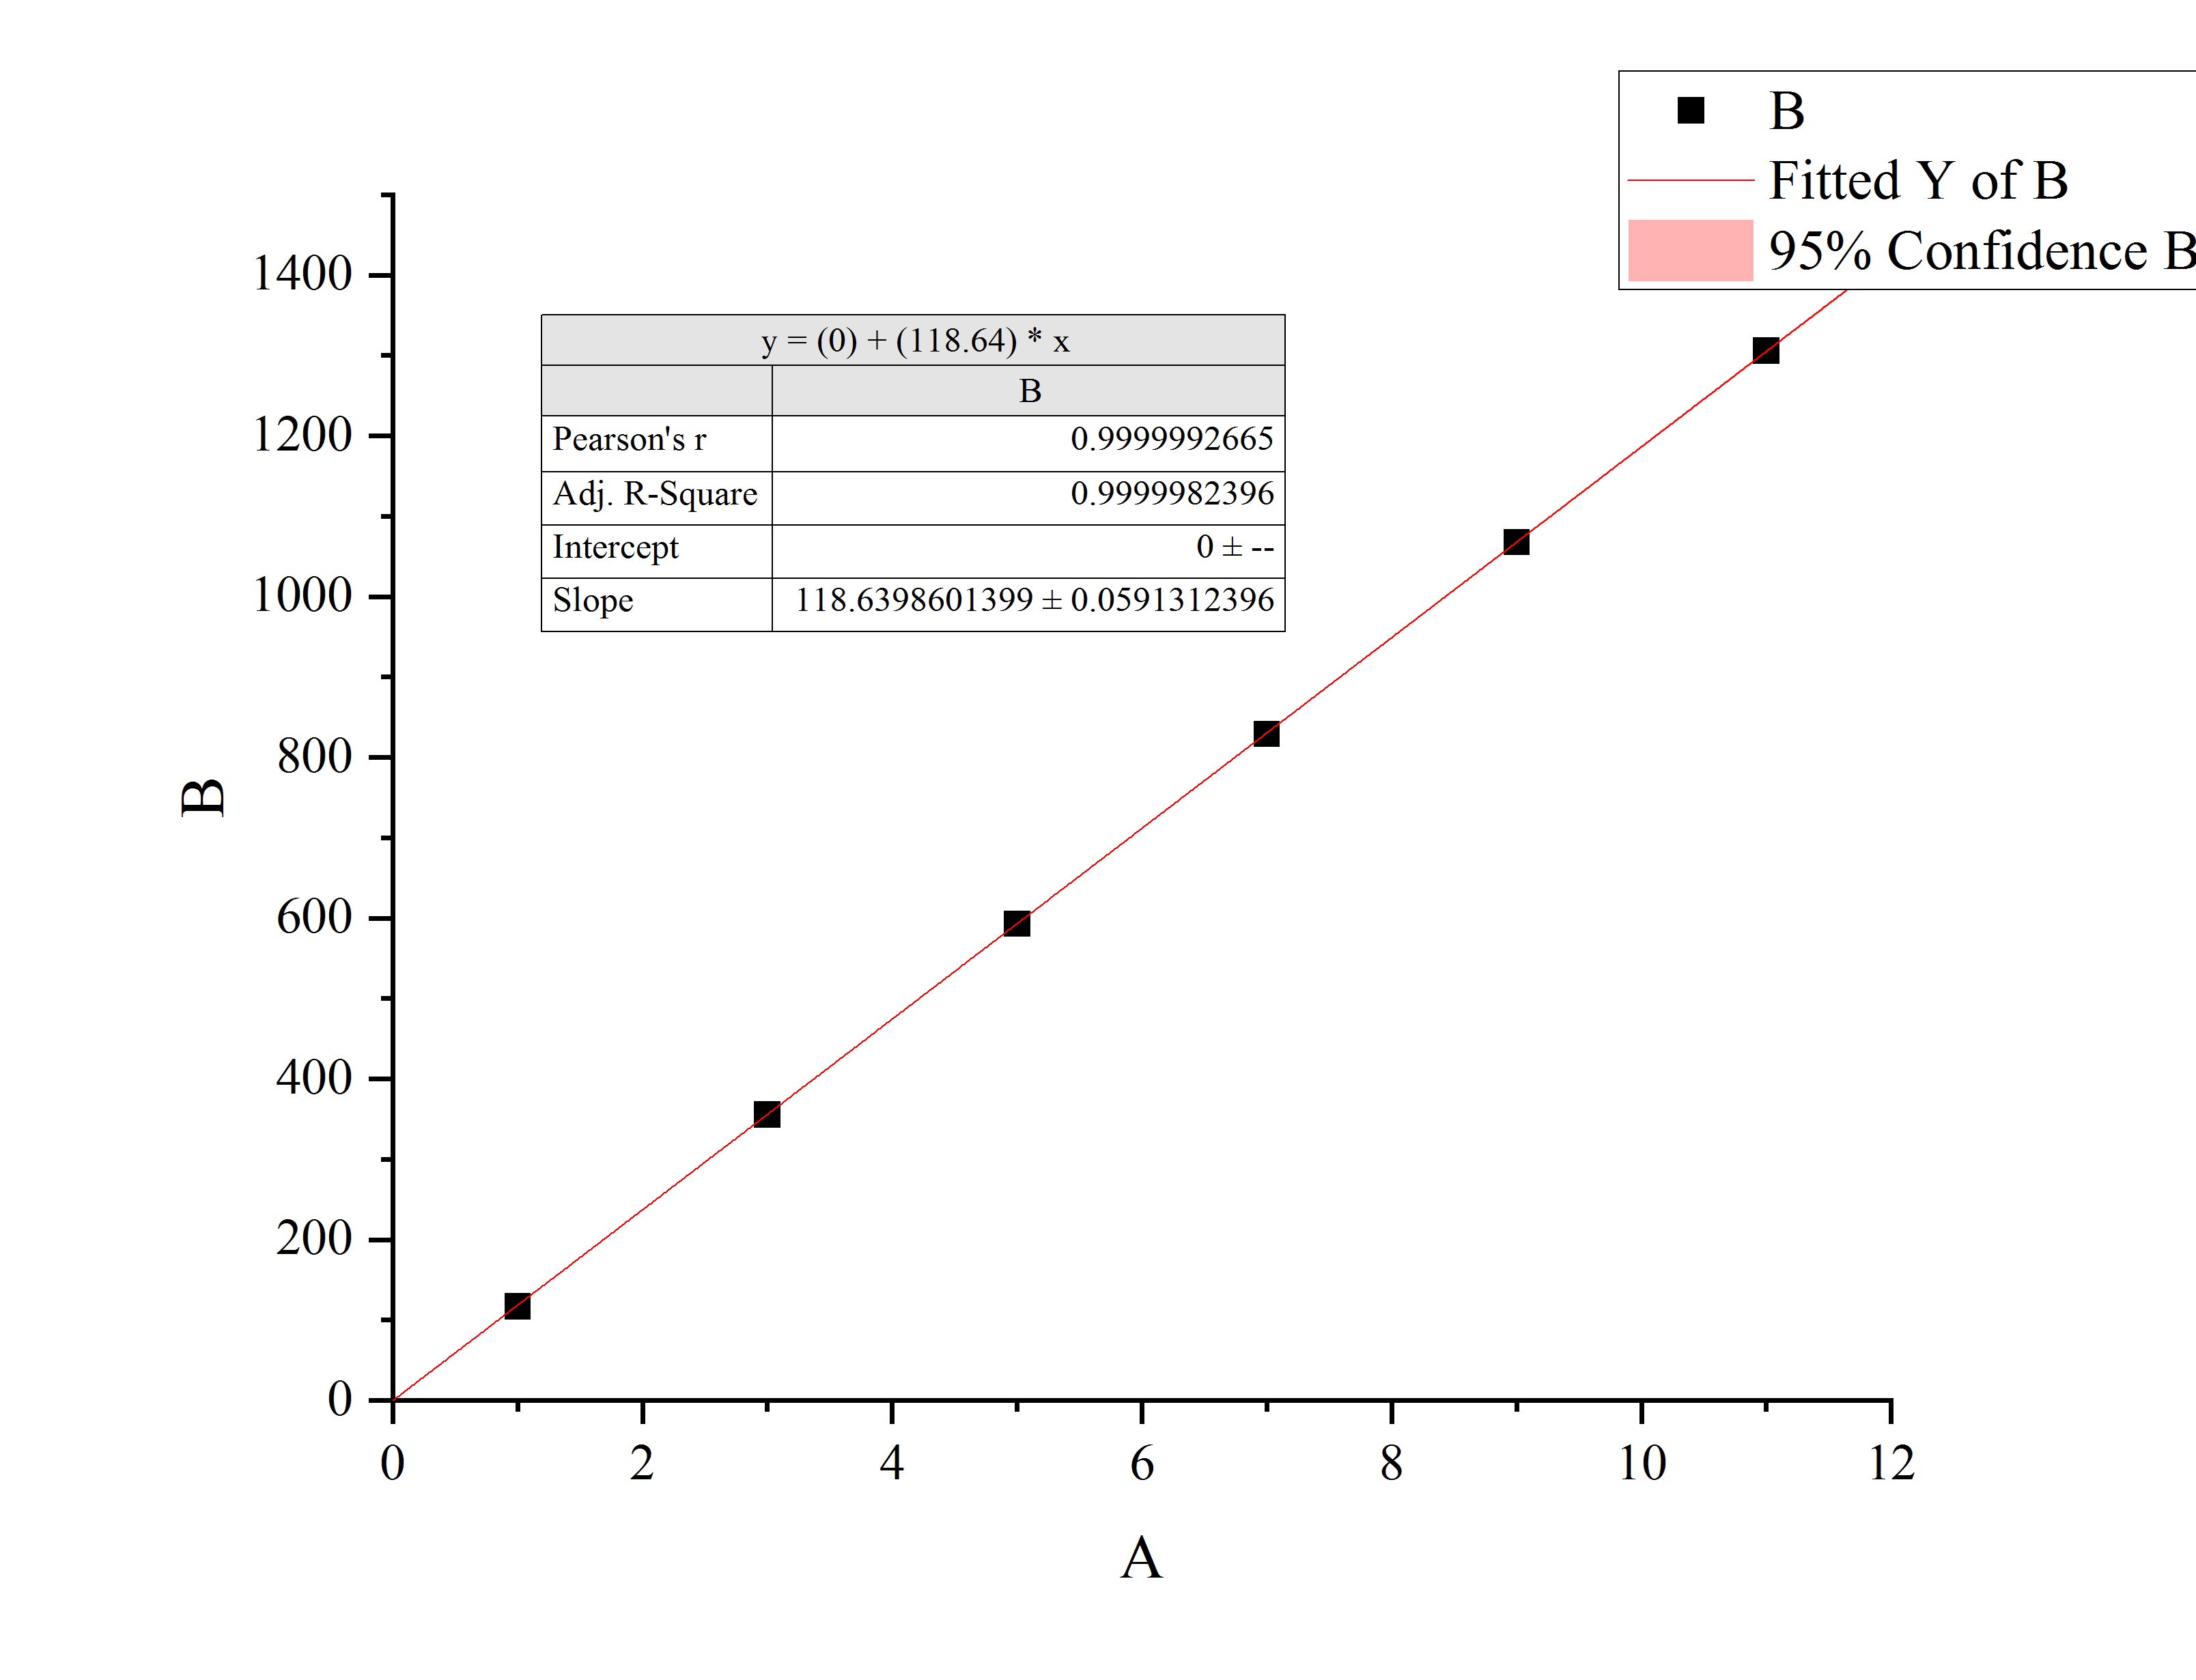
\includegraphics[trim={2.1cm 0.7cm 2.1cm 2cm},clip,width=0.47\textwidth]{img/l4.png}}\hfil
\end{figure}

\subsection{Conclusioni}

Come è possibile osservare comparando questi risultati a
quelli precedentemente ottenuti, il valore di $g$ risultante
è rimasto essenzialmente invariato (al netto della sua incertezza).

In conclusione, possiamo affermare ragionevolmente che,
rispetto alla sensibilità degli strumenti di misura,
il contributo dell'attrito è trascurabile.

\section{Misurazione diretta mediante l'eco}

\subsection{Esperienza e procedimento di misura}

\begin{enumerate}
  \item
    Posto il calorimetro sopra alla bilancia, avviamo la cattura del filmato.
  \item
    Dopo circa una decina di secondi (non è rilevante per la riuscita dell'esperienza),
    tramite il generatore forniamo calore all'azoto per mezzo della resistenza.
  \item
    Aspettato ... interrompiamo il flusso di calore e dopo
    un'altra decina di secondi terminiamo la registrazione video.
\end{enumerate}

\subsection{Analisi dei dati raccolti}
\emph{\textbf{Nota.}
Avendo valutato gli errori sulle grandezze misurate direttamente
come piccoli, casuali e indipendenti, per svolgere ogni calcolo
abbiamo utilizzato la tradizionale propagazione degli errori.
}

  Grazie al filmato possiamo graficare la variazione della massa in funzione del tempo
  e, successivamente, costruire tre distinte rette di regressione.

  Essendo note, oltre all'intervallo di tempo, tensione ed intensità della corrente,
  è nota anche la quantità di calore fornito: $Q = I \Delta V \Delta t$.

  Il calore latente dell'azoto liquido sarà:

\subsection{Conclusioni}

Come è possibile osservare comparando questi risultati a
quelli precedentemente ottenuti, il valore di $g$ risultante
è rimasto essenzialmente invariato (al netto della sua incertezza).

In conclusione, possiamo affermare ragionevolmente che,
rispetto alla sensibilità degli strumenti di misura,
il contributo dell'attrito è trascurabile.

\end{document}
